\documentclass{article}

\usepackage{amsmath}

\usepackage{graphicx}
\graphicspath{ {../outputs/} }

\usepackage{biblatex}
\bibliography{citations}

\begin{document}

  \title{Linear Time Generation of Simulated Wireless Sensor Networks with Random Geometric Graphs}
  \author{Luke Wood}
  \maketitle

  \section{Executive Summary}
	Wireless Sensor Networks can be incredibly expensive to deploy and test which makes them an excellent candidate for simulated testing.
	Vlady Ravelomananana and Hichem Kenniche from the University of Paris first explored the concept of using random geometric graphs to attempt to model wireless sensor networks \cite{kenniche2010random}.
	In this report I will describe the implementation I have created for a linear time algorithm to generate graphs consisting of N vertices with an average degree of A on the geometric topologies of: unit square, unit disc, unit sphere.
  \subsection{Introduction and Summary}
	The most powerful part of my implementation is the highly maintainable code combined with strong performance.
	As a functional programming enthusiast, I first wished to use Elixir to solve this problem but quickly realized that the enforcement of immutability by the erlangVM would be problematic going forward.
	Due to the need for mutable data I decided to go with python for my implementation of part one.
	Despite choosing to use python, I really dislike the style most python programmers use and find it ambiguous and confusing in many cases.
	To counteract this, I employed functional programming patterns inside my python implementation such as decoupling all of my code as much as possible, explicitly importing modules for the function they are used in, and avoiding branching on conditionals whenever possible.
	I believe that these helped me create low bug code.
  \subsection{Programming Environment Description}
	I developed and tested this program on a 15 inch Macbook 2017 with an i7 processor and 16 GB of ram.
  \section{Reduction to Practice}

  In order to ensure that average degree of the nodes is close to the desired average degree we define a radius surrounding each node.
  The formulas to find the radius for each topology is derived from the equations found in the paper Bipartite Grid Partitioning of a Random Geometric Graph\cite{chen2017bipartite}.
  The formula used to find this radius varies for each graph tolopogy and can be found in the table displayed below:

  \begin{tabular}{ |c|c|c| }
	  \hline
	  Topology & Equation in Chen's Paper & Equation for Radius Derive from Chen's \\
	  \hline
	  Unit Square & $d(G) \approx N\pi r^2 $ & $r = sqrt(\dfrac{d(G)}{N\pi})$ \\ 
	  \hline
	  Unit Disc   & & \\
	  \hline
	  Unit Sphere & & \\
	  \hline
  \end{tabular}

  \begin{figure}[!htb]
    \centering
    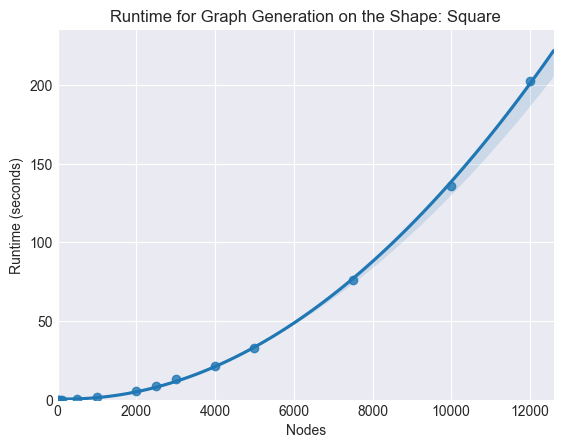
\includegraphics[width=1 \textwidth]{square/runtime/runtime_chart_naive}
    \caption{Data on the Runtime of the $O(n^2)$ Algorithm}
  \end{figure}

  \begin{figure}[!htb]
    \centering
    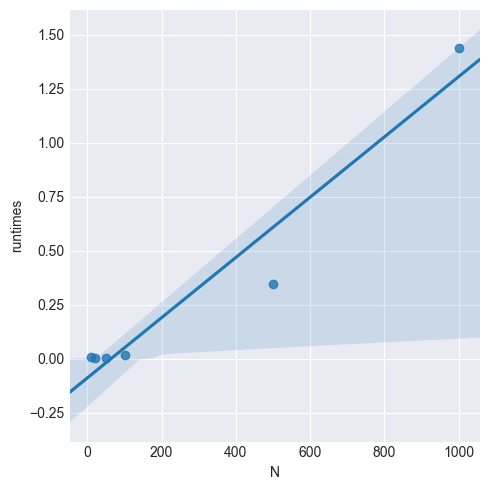
\includegraphics[width=1 \textwidth]{square/runtime/runtime_chart}
    \caption{Data on the Runtime of the $O(n)$ Algorithm}
  \end{figure}

\section{Result Summary}
  The algorithm I created is clearly $O(n)$

\printbibliography

\end{document}
